
%(BEGIN_QUESTION)
% Copyright 2005, Tony R. Kuphaldt, released under the Creative Commons Attribution License (v 1.0)
% This means you may do almost anything with this work of mine, so long as you give me proper credit

Suppose you needed to choose a fixed resistor value ($R$) to make a voltage divider circuit, given a known potentiometer resistance value, the source voltage value, and the desired range of adjustment:

$$\includegraphics[width=15.5cm]{i03131x01.eps}$$

Solve for $R$, and show the equation you set up in order to do it.  Also, determine the respective potentiometer wiper positions at 0 volts and at 17 volts.

\vfil 

\underbar{file i03131}
\eject
%(END_QUESTION)





%(BEGIN_ANSWER)

This is a graded question -- no answers or hints given!

%(END_ANSWER)





%(BEGIN_NOTES)

We may use the voltage divider formula to solve for $R$:

$$17 = 24 \left(50000 \over {50000 + R} \right)$$

$$17 (50000 + R) = 24 (50000)$$

$$850000 + 17R = 1200000$$

$$17R = 350000$$

$$R = 20.588 \hbox{ k} \Omega $$

\vskip 10pt

The potentiometer wiper will be fully {\it up} at 0 volts and fully {\it down} at 17 volts.

%INDEX% Mathematics review: manipulating literal equations

%(END_NOTES)


